\documentclass[handout]{beamer}

\usetheme[progressbar=frametitle]{metropolis}
\metroset{block=fill}

\subtitle{NTIN071 Automata and Grammars}
\author{Jakub Bulín (KTIML MFF UK)}

\date{Spring 2025\\ 
    \vspace{1in} 
    \begin{flushleft}
        \it \footnotesize * Adapted from the Czech-lecture slides by Marta Vomlelová with gratitude. The translation, some modifications, and all errors are mine.
    \end{flushleft}
}

%% packages

\usepackage{amsmath}
\usepackage{amssymb}
\usepackage{amsthm}
\usepackage{cancel}
\usepackage{color}
\usepackage{colortbl}
\usepackage{forest}
\usepackage[utf8x]{inputenc}
\usepackage{multicol}
\usepackage{multirow}

%% colors
\definecolor{Gray}{gray}{0.9}

%% TikZ
\usepackage{tikz}
    \usetikzlibrary{
        automata,
        arrows,
        backgrounds,
        decorations.pathmorphing,
        fit,
        positioning,
        shapes,
        shapes.geometric,
        tikzmark
    } 
    \tikzset{>=stealth',shorten >=1pt,auto,node distance=2cm}
    \tikzset{initial text={}}
    \tikzset{elliptic state/.style={draw,ellipse}}

%% amsthm
\theoremstyle{plain}
    \newtheorem*{algorithm}{Algorithm}    
    \newtheorem*{observation}{Observation}
    \newtheorem*{proposition}{Proposition}

\theoremstyle{remark}
    \newtheorem*{exercise}{Exercise}
    \newtheorem*{remark}{Remark}

%% macros
\DeclareMathOperator{\RegE}{RegE}
\DeclareMathOperator{\RL}{RL}

% Just for Lecture 2
\newcommand{\x}{$\times$}
\newcommand{\nx}{\ }



\title{Lecture 4 -- Regular expressions, Kleene's theorem, string substitution}


\begin{document}


\frame{\titlepage}


\begin{frame}{Recap of Lecture 3}

    \begin{itemize}
        \item Nondeterministic finite automata (NFA): can `guess' the right path to accepting, computation described by a state tree.
        \item $\epsilon$-transitions: allow to change states without reading any input
        \item Subset construction: every NFA and $\epsilon$-NFA is equivalent to a DFA (but can be easier to design, much smaller).
        \item Regular languages are closed under set operations (union, intersection, complement, difference)
        \item And under string operations (concatenation, iteration and positive iteration, reverse, left and right quotient)
    \end{itemize}

\end{frame}


\section{1.8 Regular expressions}


\begin{frame}{Regular expressions (RE)}
    
    \begin{itemize}
        \item an algebraic description of languages
        \item declarative: express the form of the words we want to accept
        \item can describe all, and only, regular languages
        \item can be viewed as a programming language, a user/friendly description of a finite automaton
    \end{itemize}

    \begin{example}
    \begin{itemize}
        \item \texttt{grep} command in UNIX.
        \item Python module \texttt{re}
        \item \alert{lexical analysis}, e.g. \texttt{Flex} (description via `tokens' $\leftrightsquigarrow$ RE)
    \end{itemize}
    \end{example}

    Note: \alert{syntax analysis} needs a stronger tool, \alert{context-free grammars}

\end{frame}


\begin{frame}{The definition}
    
    A \alert{regular expression} $\alpha$ over (finite, nonempty) $\Sigma$, $\alpha\in \alert{\RegE(\Sigma)}$ and the matching language \alert{$L(\alpha)$}, are defined inductively:

    \begin{tabular}{l l l}
        \\\hline
        \textbf{expression} & \textbf{language} & \textbf{note}\\\hline
        $\emptyset$ & $L(\emptyset)=\emptyset$ & empty expression\\
        $\epsilon$ & $L(\epsilon)=\{\epsilon\}$ & empty string \\
        
        $\textbf{a}$ & $L({\bf a})=\{a\}$ & for all $a\in \Sigma$\\
         $(\alpha+\beta)$ & $L((\alpha+\beta))=L(\alpha)\cup L(\beta) $ & union (\texttt{grep}, \texttt{re} use `$|$')\\
         $(\alpha\beta)$ & $L((\alpha\beta))=L(\alpha)L(\beta)$ &concatenation \\
         $\alpha^*$ & $L(\alpha^*)=L(\alpha)^*$ & iteration (Kleene star)
    \end{tabular}
    
\end{frame}


\begin{frame}{Examples, notation}

    \begin{example}
        \begin{itemize}
            \item The language of alternating 0s and 1s can be expressed as:
            \begin{itemize}
                \item $({\bf 01})^*+({\bf 10})^*+{\bf 1}({\bf 01})^*+{\bf 0}({\bf 10})^*$
                \item $(\epsilon+{\bf 1})({\bf 01})^*(\epsilon+{\bf 0})$
            \end{itemize}
            \item $L((\textbf{0}^*\textbf{10}^*\textbf{10}^*\textbf{1})^*\textbf{0}^*)=\{w\in \{0,1\}^*\mid |w|_1 \equiv 0\pmod 3\}$
        \end{itemize}
    \end{example}

    We often omit parentheses:
    \begin{itemize}
        \item priority of operators: iteration $*$ $>$ concatenation $>$ union $+$
        \item associativity of concatenation, union $+$
        \item outer parentheses
    \end{itemize}

    We could define, and will sometimes use, positive iteration $\alpha^+$

\end{frame}


\begin{frame}{Kleene's theorem}

    \begin{theorem}[Kleene's theorem]
        A language is regular, iff it is matched by some regular expression.
    \end{theorem}

    We will prove it by giving two constructions:
    \begin{enumerate}
        \item from RE to $\epsilon$-NFA (which can be converted to a DFA)
		\item from a DFA to a RE (but we could start from a $\epsilon$-NFA)
	\end{enumerate}
    For 2. we also mention a better algorithm: \alert{state eliminiation}

\end{frame}


\begin{frame}{RE to $\epsilon$-NFA}

    By induction on the structure of $\alpha$, construct a $\epsilon$-NFA $E$ s.t. $L(\alpha)=L(E)$ with three additional properties:
	\begin{enumerate}
		\item Exactly one accepting state.
		\item No incoming edges into the initial state.
		\item No outgoing edges from the accepting state.
	\end{enumerate}
	
    \bigskip

	\textbf{Induction base:} $\alpha$ is the empty string $\epsilon$, empty set $\emptyset$, or a letter ${\bf a}$
	
	\begin{multicols}{3}
	
        \centering
        \begin{tikzpicture}[>=stealth',shorten >=1pt,auto,node distance=2cm,transform canvas={scale=0.95}]
            \tikzset{every state/.style={minimum size=0pt}}
            \node[initial,state] (q0)      {};
            \node[state,accepting] (q1) [right of=q0]     {};
            \path[->] (q0)  edge node {$\epsilon$} (q1);
            \node[state] (X)[rectangle,  fit= (q0) (q1), inner sep=0.3cm,rounded corners] {};
        \end{tikzpicture}	
        
        \begin{tikzpicture}[>=stealth',shorten >=1pt,auto,node distance=2cm,transform canvas={scale=0.95}]
            \tikzset{every state/.style={minimum size=0pt}}
            \node[initial,state] (q0)      {};
            \node[state,accepting] (q1) [right of=q0]     {};
            \path[->];
            \node[state] (X)[rectangle,  fit= (q0) (q1), inner sep=0.3cm,rounded corners] {};
        \end{tikzpicture}
            
        \begin{tikzpicture}[>=stealth',shorten >=1pt,auto,node distance=2cm,transform canvas={scale=0.95}]
            \tikzset{every state/.style={minimum size=0pt}}
            \node[initial,state] (q0)      {};
            \node[state,accepting] (q1) [right of=q0]     {};
            \path[->] (q0)  edge node {$a$} (q1);	
            \node[state] (X)[rectangle,  fit= (q0) (q1), inner sep=0.3cm,rounded corners] {};
        \end{tikzpicture}
	
	\end{multicols}

    \bigskip

    \textbf{Induction step:} $\alpha+\beta$, $\alpha\beta$, $\alpha^*$ (next slide) \hfill\qedsymbol
	
\end{frame}


\begin{frame}{RE to $\epsilon$-NFA: Induction step}
    
    \vspace{-1cm}
    Let $A,B$ be $\epsilon$-NFA constructed for $\alpha,\beta$.

    \bigskip

    Addition $\alpha+\beta$

    \vspace{-1cm}

	\hspace{0.4\textwidth}\begin{tikzpicture}[>=stealth',shorten >=1pt,auto,node distance=2cm,transform canvas={scale=0.8}]
		\tikzset{every state/.style={minimum size=0pt}}
		\node[initial,state] (q0)      {};
		\node[state] (q1a)   [right of=q0]    {};
		\node[state] (q1b)   [below of=q1a]    {};
		\node[state] (q2a)   [draw=none,right of=q1a]    {A};
		\node[state] (q2b)   [draw=none,right of=q1b]    {B};
		\node[state] (q3a)  [right of=q2a]     {};
		\node[state] (q3b)  [right of=q2b]     {};
		\node[state,accepting] (q1) [right of=q3a]     {};
		\path[->]
			(q0)  edge node {$\epsilon$} (q1a)
			(q0)  edge node {$\epsilon$} (q1b)
			(q3a)  edge node {$\epsilon$} (q1)
			(q3b)  edge node {$\epsilon$} (q1)
		;
		\node[state] (X)[rectangle,  fit= (q1a) (q3a), inner sep=0.3cm,rounded corners] {};
		\node[state] (Y)[rectangle,  fit= (q1b) (q3b), inner sep=0.3cm,rounded corners] {};
	\end{tikzpicture}

    \vfill\vfill

    Concatenation $\alpha\beta$	

	\hspace{0.4\textwidth}\begin{tikzpicture}[>=stealth',shorten >=1pt,auto,node distance=1cm,transform canvas={scale=0.8}]
		\tikzset{every state/.style={minimum size=0pt}}
		\node[initial,state] (q1a)      {};
		\node[state] (q2a)   [draw=none,right of=q1a]    {A};
		\node[state] (q3a)  [right of=q2a]     {};
		\node[state] (q1b)   [right=2cm of q3a]    {};
		\node[state] (q2b)   [draw=none,right of=q1b]    {B};
		\node[state,accepting] (q3b)  [right of=q2b]     {};
		\path[->]
			(q3a)  edge node {$\epsilon$} (q1b)
		;
	    \node[state] (X)[rectangle,  fit= (q1a) (q3a), inner sep=0.3cm,rounded corners] {};
		\node[state] (Y)[rectangle,  fit= (q1b) (q3b), inner sep=0.3cm,rounded corners] {};
	\end{tikzpicture}
			
    \vfill

	Iteration $\alpha^*$

	\hspace{0.4\textwidth}\begin{tikzpicture}[>=stealth',shorten >=1pt,auto,node distance=2cm,transform canvas={scale=0.8}]
		\tikzset{every state/.style={minimum size=0pt}}
		\node[initial,state] (q0)      {};
		\node[state] (q2)   [right of=q0]    {};
		\node[state] (q4)   [draw=none,right of=q2]    {A};
		\node[state] (q3)  [right of=q4]     {};
		\node[state,accepting] (q1) [right of=q3]     {};
		\path[->]
			(q0)  edge node {$\epsilon$} (q2)
			(q3)  edge node {$\epsilon$} (q1)
			(q3)  edge[bend right,swap] node {$\epsilon$} (q2)
			(q0)  edge[bend right,swap] node {$\epsilon$} (q1)
		;
		\node[state] (X)[rectangle,  fit= (q2) (q3), inner sep=0.3cm,rounded corners] {};
	\end{tikzpicture}
    
\end{frame}


\begin{frame}{DFA to RE}

    Assume the states are  $Q=\{1,\ldots,n\}$ and the start state is $q_0=1$. 
    
    Construct a RE \alert{$R_{ij}^{(k)}$} matching words that transition from state $i$ into state $j$ and all intermediate states (if any) have index $\leq k$.

    Then we set \alert{$\alpha=\sum_{j\in F_A}R_{1j}^{(n)}$} (from start to some accepting state)

    Iteratively construct $R_{ij}^{(k)}$ for $k=0,\ldots,n$ (finite induction).

    \textbf{Induction base:} $k=0$
    \begin{itemize}
        \item If \alert{$i\neq j$}, set $R_{ij}^{(0)}={\bf a_1}+\ldots+{\bf a_m}$ where $a_1,\dots,a_m$ are symbols on edges from $i$ into $j$ ($R_{ij}^{(0)}=\emptyset$ or $R_{ij}^{(0)}={\bf a}$ for $m=0,1$).
        \item If \alert{$i=j$}, $R_{ii}^{(0)}=\alert{\epsilon+}{\bf a_1}+\ldots+{\bf a_m}$ where $a_i$'s are on loops on $i$.
    \end{itemize}

\end{frame}


\begin{frame}{DFA to RE: Induction step}

    Once we have $ R^{(k)}_{ij}$ for all $i,j\in Q$, we can construct $R^{(k+1)}_{ij}$:
        
    $$
    R^{(k+1)}_{ij}=R^{(k)}_{ij}+ R^{(k)}_{i(k+1)}(R^{(k)}_{(k+1)(k+1)})^*R^{(k)}_{(k+1)j}
    $$

    \bigskip

    \begin{center}
        \scalebox{0.85}{
            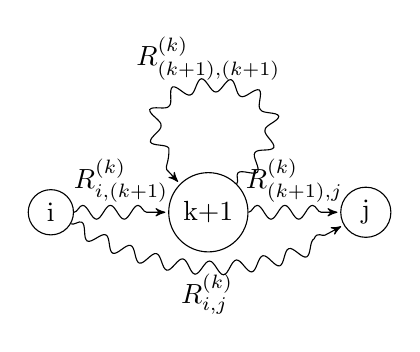
\begin{tikzpicture}
                \tikzset{every state/.style={minimum size=0.2cm}}
                \node[state] (a) at (12,0.5)     {i};
                \node[state] (g)  [right of=a]     {k+1};
                \node[state] (g2)  [right of=g]     {j};
                \path[->]
                    (a)  edge[decorate,decoration={snake,post length=2mm}]  node {$R^{(k)}_{i,(k+1)}$} (g)
                    (g)  edge[decorate,decoration={snake,post length=2mm}]  node {$R^{(k)}_{(k+1),j}$} (g2)
                    (a)  edge[decorate,decoration={snake,post length=2mm}, bend right,swap]  node {$R^{(k)}_{i,j}$} (g2)
                    (g)  edge[loop=110,decorate,decoration={snake,post length=2mm},swap]  node {$R^{(k)}_{(k+1),(k+1)}$} (g);     
            \end{tikzpicture}
        }            
    \end{center}

    \vspace{-12pt}

    \begin{itemize}
        \item paths $i\rightsquigarrow j$ not going through $k+1$: already in $R^{(k)}_{ij}$
        \item paths $i\rightsquigarrow j$ going through $k+1$ one or more times: $i\rightsquigarrow k+1$ (first visit), loop on $k+1$, finally  (last visit) $k+1\rightsquigarrow j$\hfill\qedsymbol
    \end{itemize}

\end{frame}


\begin{frame}{Example}

    \begin{multicols*}{2}

        \begin{center}
            \scalebox{0.9}{
                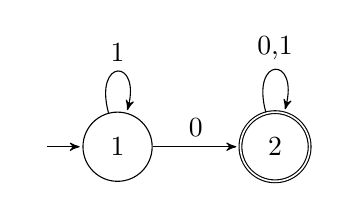
\begin{tikzpicture}[>=stealth',shorten >=1pt,auto,node distance=2cm]
                    \node[initial,state] (q1)      {1};
                    \node[state,accepting] (q2) [right of=q1]     {2};
                    \path[->]
                        (q1)  edge[loop above]  node {1} (q1)
                        (q1)  edge  node {0} (q2)
                        (q2)  edge[loop above] node {0,1} (q2);
                \end{tikzpicture}
            }    
        
        \vspace{2cm}

        Apply the construction, simplify:

        $\alpha=R_{12}^{(2)}={\bf 1}^*{\bf 0}({\bf 0}+{\bf 1})^*$
        
        

    \end{center}

    \end{multicols*}
        
    

    \begin{center}\footnotesize
        \begin{tabular}{r | l @{=} l}
        %& By direct substitution &Simplified\\
        $R_{11}^{(0)}$ & $\epsilon +{\bf 1}$ &\\
        $R_{12}^{(0)}$ & ${\bf 0}$&\\ 
        $R_{21}^{(0)}$ & $\emptyset$&\\
        $R_{22}^{(0)}$ & $(\epsilon +{\bf 0}+{\bf 1})$&\\
        \hline
        $R_{11}^{(1)}$ & $\epsilon +{\bf 1}+(\epsilon +{\bf 1})(\epsilon +{\bf 1})^*(\epsilon +{\bf 1})$ & ${\bf 1}^*$\\
        $R_{12}^{(1)}$ & ${\bf 0} +(\epsilon +{\bf 1})(\epsilon +{\bf 1})^*{\bf 0}$ &  ${\bf 1}^*{\bf 0}$\\
        $R_{21}^{(1)}$ & $\emptyset +\emptyset(\epsilon +{\bf 1})^*(\epsilon +{\bf 1})$&$\emptyset$\\
        $R_{22}^{(1)}$ & $\epsilon+{\bf 0} +{\bf 1}+\emptyset(\epsilon +{\bf 1})^*{\bf 0}$&$\epsilon+{\bf 0}+{\bf 1}$\\ 
        \hline
        $R_{11}^{(2)}$ & ${\bf 1}^*+{\bf 1}^*{\bf 0}(\epsilon +{\bf 0}+{\bf 1})^*\emptyset$ & ${\bf 1}^*$\\
        $R_{12}^{(2)}$ & ${\bf 1}^*{\bf 0}+{\bf 1}^*{\bf 0}(\epsilon +{\bf 0}+{\bf 1})^*(\epsilon +{\bf 0}+{\bf 1})$ & ${\bf 1}^*{\bf 0}({\bf 0}+{\bf 1})^*$\\
        $R_{21}^{(2)}$ & $\emptyset+(\epsilon +{\bf 0}+{\bf 1})(\epsilon +{\bf 0}+{\bf 1})^*\emptyset$ & $\emptyset$\\
        $R_{22}^{(2)}$ & $\epsilon+{\bf 0}+{\bf 1}+(\epsilon +{\bf 0}+{\bf 1})(\epsilon +{\bf 0}+{\bf 1})^*(\epsilon +{\bf 0}+{\bf 1})$ & $({\bf 0}+{\bf 1})^*$
        \end{tabular}
    \end{center}

\end{frame}


\section*{State elimination algorithm}

\begin{frame}{State elimination: the idea}

    \textbf{Idea:} Allow edges labelled by RE, iteratively remove nodes. (More efficient, avoids duplicity.) 
	
	\begin{multicols}{2}
	
        \begin{center}
            \it State $s$ selected for elimination        
            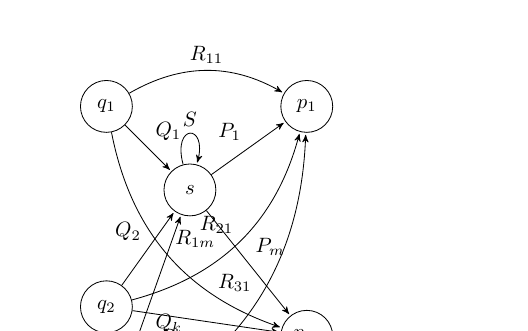
\begin{tikzpicture}[]
                \useasboundingbox (-1,-2.50) rectangle (5,1);
                \scope[transform canvas={scale=0.75}]
                \node[state] (q1)      {$q_1$};
                \node[state] (p1)  [right=2.5cm of q1]     {$p_1$};
                \node[state] (s)  [below right of=q1]    {$s$};
                \node[state] (q2)  [below=2.5cm of q1]     {$q_2$};
                \node[state] (qk)  [below of=q2]     {$q_k$};
                \node[state] (pm)  [below=3cm of p1]     {$p_m$};
                \path[->]
                    (q1)  edge [bend left] node {$R_{11} $} (p1)
                    (q1)  edge [bend right] node {$R_{1m} $} (pm)
                    (q2)  edge [bend right] node {$R_{21} $} (p1)
                    (q2)  edge [swap] node {$R_{2m} $} (pm)
                    (qk)  edge [bend right] node {$R_{31} $} (p1)
                    (qk)  edge [swap] node {$R_{3m} $} (pm)
                    (q1)  edge  node {$Q_{1} $} (s)
                    (q2)  edge  node {$Q_{2} $} (s)
                    (qk)  edge [swap] node {$Q_{k} $} (s)
                    (s)  edge  node {$P_{1} $} (p1)
                    (s)  edge  node {$P_{m} $} (pm)
                    (s)  edge[loop above]  node {$S$} (s);
                \endscope
            \end{tikzpicture}
        \end{center}
	
	    \begin{center}
	        \it After $s$ is eliminated.	
            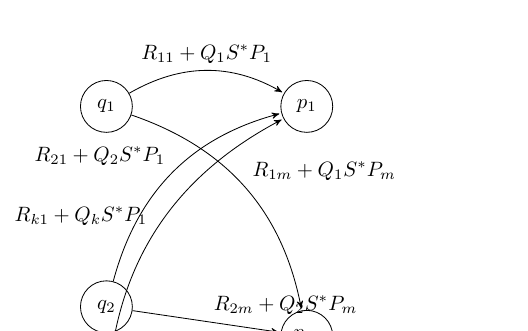
\begin{tikzpicture}[]
                \useasboundingbox (-1,-2.50) rectangle (5,1);
                \scope[transform canvas={scale=0.75}]
                \node[state] (q1)      {$q_1$};
                \node[state] (p1)  [right=2.5cm of q1]     {$p_1$};
                \node[state] (q2)  [below=2.5cm of q1]     {$q_2$};
                \node[state] (qk)  [below of=q2]     {$q_k$};
                \node[state] (pm)  [below=3cm of p1]     {$p_m$};
                \path[->]
                    (q1)  edge [bend left] node {$R_{11}+Q_{1} S^* P_{1} $} (p1)
                    (q1)  edge [bend left] node {$R_{1m}+Q_{1} S^* P_{m} $} (pm)
                    (q2)  edge [bend left] node {$R_{21}+Q_{2} S^* P_{1} $} (p1)
                    (q2)  edge  node {$R_{2m}+Q_{2} S^* P_{m} $} (pm)
                    (qk)  edge [bend left] node {$R_{k1}+Q_{k} S^* P_{1} $} (p1)
                    (qk)  edge [swap] node {$R_{km}+Q_{k} S^* P_{m} $} (pm);
                \endscope
            \end{tikzpicture}
        \end{center}
	
	\end{multicols}

\end{frame}


\begin{frame}{State elimination: the algorithm}
    
    For every accepting $q\in F$ eliminate all states $p\in Q\setminus\{q, q_0\}$.
    \begin{itemize}
        \item for $q\neq q_0$: \alert{$\RegE(q)=(R+SU^*T)^*SU^*$}
            \begin{center}
                \scalebox{0.8}{
                    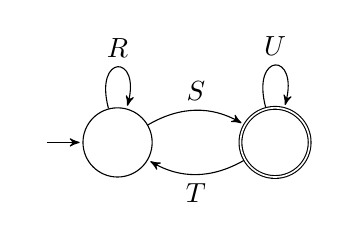
\begin{tikzpicture}[>=stealth',shorten >=1pt,auto,node distance=2cm]
                        \node[initial,state] (q1)      {};
                        \node[state,accepting] (q2) [right of=q1] {};
                        \path[->]
                            (q1)  edge[loop above]  node {$R$} (q1)
                            (q1)  edge[bend left]  node {$S$} (q2)
                            (q2)  edge[bend left]  node {$T$} (q1)
                            (q2)  edge[loop above] node {$U$} (q2);
                    \end{tikzpicture}
                }
            \end{center}
            

        \item for $q= q_0$: \alert{$\RegE(q)=R^*$}
            \begin{center}
                \scalebox{0.8}{
                    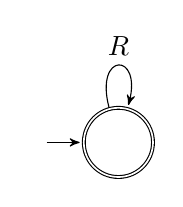
\begin{tikzpicture}[>=stealth',shorten >=1pt,auto,node distance=2cm]
                        \node[initial,state,accepting] (q1) {};
                        \path[->] (q1)  edge[loop above]  node {$R$} (q1);
                    \end{tikzpicture}
                }
            \end{center}
    \end{itemize}
    Finally, union over all accepting states: \alert{$\RegE(A)=\sum_{q\in F}\RegE(q)$}

    \medskip

    (Elimination order: first nonaccepting and noninitial states.)

\end{frame}


\begin{frame}{State elimination: an example}

    The original automaton: 

	\hspace{5cm}
    
\begin{tikzpicture}[>=stealth',shorten >=1pt,auto,node distance=2cm,transform canvas={scale=0.8}]
        \node[initial,state] (q0)      {A};
        \node[state] (q1)  [right of=q0]     {B};
        \node[state,accepting] (q2)  [right of=q1]     {C};
        \node[state,accepting] (q3) [right of=q2]     {D};
        \path[->]
            (q0)  edge[loop above]  node {0,1} (q0)
            (q0)  edge  node {1} (q1)
            (q1)  edge node {0,1} (q2)
            (q2)  edge node {0,1} (q3);
    \end{tikzpicture}
	
	Replace letters by RE: 
		
	\vspace{0.4cm}\hspace{5cm}
	
\begin{tikzpicture}[>=stealth',shorten >=1pt,auto,node distance=2cm,transform canvas={scale=0.8}]
		\node[initial,state] (q0)      {A};
		\node[state] (q1)  [right of=q0]     {B};
		\node[state,accepting] (q2)  [right of=q1]     {C};
		\node[state,accepting] (q3) [right of=q2]     {D};
		\path[->]
			(q0)  edge[loop above]  node {{\bf 0}+{\bf 1}} (q0)
			(q0)  edge  node {{\bf 1}} (q1)
			(q1)  edge node {{\bf 0}+{\bf 1}} (q2)
			(q2)  edge node {{\bf 0}+{\bf 1}} (q3);
	\end{tikzpicture}
			
	Eliminate B: 
		
	\vspace{0.4cm} 
	\hspace{5cm}
	\begin{tikzpicture}[>=stealth',shorten >=1pt,auto,node distance=2cm,transform canvas={scale=0.8}]
		\node[initial,state] (q0)      {A};
		\node[state,accepting] (q2)  [right of=q1]     {C};
		\node[state,accepting] (q3) [right of=q2]     {D};
		\path[->]
			(q0)  edge[loop above]  node {{\bf 0}+{\bf 1}} (q0)
			(q0)  edge node {{\bf 1}({\bf 0}+{\bf 1})} (q2)
			(q2)  edge node {{\bf 0}+{\bf 1}} (q3);
	\end{tikzpicture}
			
	Eliminate C:
	
    \vspace{0.4cm}
	\hspace{5cm}
	\begin{tikzpicture}[>=stealth',shorten >=1pt,auto,node distance=2cm,transform canvas={scale=0.8}]
		\node[initial,state] (q0)      {A};
		\node[state,accepting] (q3) [right of=q2]     {D};
		\path[->]
			(q0)  edge[loop above]  node {{\bf 0}+{\bf 1}} (q0)
			(q0)  edge node {{\bf 1}({\bf 0}+{\bf 1})({\bf 0}+{\bf 1})} (q3);
	\end{tikzpicture}

    \vspace{-0.2cm}
	$$
    ({\bf 0}+{\bf 1})^*{\bf 1}({\bf 0}+{\bf 1})+({\bf 0}+{\bf 1})^*{\bf 1}({\bf 0}+{\bf 1})({\bf 0}+{\bf 1})
    $$
	
\end{frame}


\begin{frame}{Algebraic description of regular languages}

    Let \alert{$\RL(\Sigma)$} denote the smallest set of languages over $\Sigma$ that:
    \begin{itemize}
        \item contains $\emptyset$ and $\{x\}$ for any letter $x\in \Sigma$, and 
        \item is closed under union, concatenation, and iteration.
    \end{itemize}
    That is, for $A,B\in \RL(\Sigma)$ also $A\cup B,A.B,A^*\in \RL(\Sigma)$. Note that:

    \begin{itemize}
        \item $\{\epsilon\}\in\RL(\Sigma)$ since $\{\epsilon\}=\emptyset^*$
        \item $\Sigma\in\RL(\Sigma)$ since $\Sigma=\bigcup_{x\in \Sigma}\{x\}$ (a finite union)
        \item $\Sigma^*\in\RL(\Sigma)$
        \item any finite language over $\Sigma$ is in $\RL(\Sigma)$.
    \end{itemize}
        
    \bigskip
        
    \begin{theorem}[A restatement of Kleene's Theorem]
        A language over $\Sigma$ is regular, iff it is in $\RL(\Sigma)$.
    \end{theorem}    

\end{frame}


\begin{frame}{Some properties to simplify RE  (will not be tested)}

    \begin{eqnarray*}
        L.\emptyset=\emptyset.L&=&\emptyset\\
        \{\epsilon\}.L=L.\{\epsilon\}&=& L\\
        (L^*)^* &=& L^*\\
        (L_1\cup L_2)^*&=& L_1^*(L_2.L_1^*)^*=L_2^*(L_1.L_2^*)^*\\
        (L_1.L_2)^R&=&L_2^R.L_1^R\\
        \partial_w(L_1\cup L_2)&=&\partial_w(L_1)\cup \partial_w(L_2)\\
        \partial_w(\Sigma^*-L)&=&\Sigma^*-\partial_w L\hbox{.}
    \end{eqnarray*}

\end{frame}


\begin{frame}{Converting between representations}

    \begin{center}
        \scalebox{0.8}{
            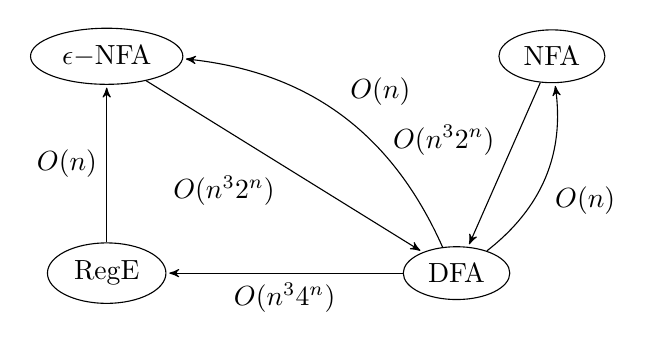
\begin{tikzpicture}
                \node[elliptic state] (q0)      {$\epsilon-$NFA};
                \node[elliptic state] (q1)  [right=4cm of q0]     {NFA};
                \node[elliptic state] (q2)  [below=2cm of q0]     {RegE};
                \node[elliptic state] (q3) [right=3cm of q2]     {DFA};
                \path[->]
                    (q0)  edge  node[swap] {$O(n^3 2^n )$} (q3)
                    (q1)  edge  node[swap] {$O(n^3 2^n )$} (q3)
                    (q2)  edge node {$O(n)$} (q0)
                    (q3)  edge node {$O(n^3 4^n)$} (q2)
                    (q3)  edge[bend right] node[swap] {$O(n)$} (q0)
                    (q3)  edge[bend right] node[swap] {$O(n)$} (q1)
                    ;
            \end{tikzpicture}
        }
    \end{center}
        
    \begin{itemize}
        \item NFA or $\epsilon$-NFA to DFA: $O(n^32^n)$
        \begin{itemize}
            \item $\epsilon$-closure in $O(n^3)$ (search $n$ states $\times$ $n^2$ arcs)
            \item subset construction, DFA with up to $2^n$ states; for each state need $O(n^3)$ time to compute transitions.
        \end{itemize}        
        \item DFA to NFA or $\epsilon$-NFA: $O(n)$
        \begin{itemize}
            \item a simple modification of the transition table
        \end{itemize}        
        \item DFA to RE:  $O(4^n)$        
        \item RE to $\epsilon$-NFA: $O(n)$        
    \end{itemize}

\end{frame}


\section*{String substitution}


\begin{frame}{String substitution and homomorphism}
   
    A (string) \alert{substitution} is a mapping $\sigma\colon \Sigma^*\rightarrow \mathcal P(Y^*)$ where
    \begin{itemize}
        \item $\Sigma$ and $Y$ are finite alphabets, $Y=\bigcup_{x\in \Sigma}Y_x$
        \item for each $x\in \Sigma$, $\sigma(x)$ is a language over $Y_x$
        \item $\sigma(\epsilon)=\{\epsilon\}$ and $\sigma(u.v)=\sigma(u).\sigma(v)$
    \end{itemize}
    For a language $L\subseteq \Sigma^*$, $\alert{\sigma(L)}=\bigcup_{w\in L}\sigma(w)\subseteq Y^*$. A substitution is \alert{$\epsilon$-free} if no $\sigma(x)$ contains $\epsilon$.

    A (string) \alert{homomorphism} is defined similarly but each letter is mapped to a single word, $h\colon\Sigma^*\rightarrow Y^*$ where $h(x)\in Y_x^*$ for $x\in\Sigma$, $h(\epsilon)=\epsilon$ and $h(u.v)=h(u).h(v)$. Then \alert{$h(L)=\{h(w)\mid w\in L\}$}. It is \alert{$\epsilon$-free} if $h(x)\neq\epsilon$ for all $x\in\Sigma$.

    The \alert{inverse homomorphism} applied to a language $L'\subseteq Y^*$: 
    $$
    h^{-1}(L')=\{w\in\Sigma^*\mid h(w)\in L'\}
    $$

\end{frame}


\begin{frame}{Examples}

    \begin{example}[Substitution]        
        \begin{itemize}
            \item If $\sigma(0)=\{a^ib^j, i,j\geq 0\}$ and $\sigma(1)=\{cd\}$, then $\sigma(010)=\{a^ib^jcda^kb^l\mid i,j,k,l\geq 0\}$.
            \item $\Sigma=\{f,l,s,c,d\}$, $L=L((fsl)(cfsl)^*d)$ where         
            \begin{itemize}
                \item $\sigma(f)$ is a dictionary of first names
                \item $\sigma(l)$ are last names
                \item $\sigma(s)=\{`\ '\}$ (space), $\sigma(c)=\{`,'\}$, $\sigma(d)=\{`.'\}$
            \end{itemize}
            \item A document template with symbols to be replaced by fields of database entries.            
        \end{itemize}
    \end{example}

    \begin{example}[Homomorphism]        
        \begin{itemize}
            \item Define $h(0)=ab$ and $h(1)=\epsilon$. Then $h(0011)=abab$ and for $L={\bf 10}^*{\bf 1}$ we have $h(L)=L((ab)^*)$.
            \item Replace special symbols with {\TeX} code (e.g. $h(\mu)=\backslash mu$).            
        \end{itemize}
    \end{example}  

\end{frame}


\begin{frame}{Preserving regularity}

    \begin{theorem}
        Let $L\subseteq\Sigma^*$ be regular, $h\colon\Sigma^*\rightarrow Y^*$ a homomorphism, and $\sigma\colon \Sigma^*\rightarrow \mathcal P(Y^*)$ a substitution.
        \begin{itemize}
            \item The language $h(L)$ is regular.
            \item If $\sigma(x)$ is regular for all $x\in\Sigma$, then $\sigma(L)$ is also regular.
        \end{itemize}
        Moreover, if $L'\subseteq Y^*$ is regular, then $h^{-1}(L')$ is also regular.
    \end{theorem}

\end{frame}

        
\begin{frame}{Proof for homomorphism and substitution}

    Homomorphism $\leftrightsquigarrow$ substitution with $\sigma(x)$ one-element (regular).

    Structural induction on a RE $\alpha$ such that $L=L(\alpha)$. 
    
    \begin{itemize}
        \item \textbf{Induction base:} $\emptyset$, $\epsilon$, $\mathbf{a}$ 
        \dots easy
        \item \textbf{Induction step:}
        \begin{eqnarray*}
            \sigma(L(\alpha+\beta))&=&\sigma(L(\alpha))\cup \sigma(L(\beta))\\
            \sigma(L(\alpha \beta))&=&\sigma(L(\alpha)).\sigma(L(\beta))
        \end{eqnarray*}        
        For iteration, decompose into an infinite union of powers:
        \begin{eqnarray*}
            \sigma(L(\alpha)^*)&=&\sigma(L(\alpha)^0)\cup \sigma(L(\alpha)^1)\cup \ldots\\
            &=&\sigma(L(\alpha))^0\cup \sigma(L(\alpha))^1\cup \ldots=\sigma(L(\alpha))^*\\
            &
        \end{eqnarray*}
        
    \end{itemize}

    (Alternative view: take the tree of the RE $\alpha$ and replace every leaf $x$ with a tree for a RE for $\sigma(x)$.)\hfill\qedsymbol

\end{frame}


\begin{frame}{Proof for inverse homomorphism \& an example}

    Given a DFA $A=(Q,Y, \delta,q_0,F)$ recognizing $L'$, construct a DFA recognizing $h^{-1}(L')$: \alert{$B(Q,\Sigma, \delta_B,q_0,F)$} with \alert{$\delta_B(q,a)=\delta^*(q,h(a))$}     
    That is, for a letter $a\in\Sigma$ do what $A$ does for the word $h(a)$. Easy to show (by induction on $|w|$) that $\delta_B^*(q_0,w)=\delta^*(q_0,h(w))$.
    \begin{center}
        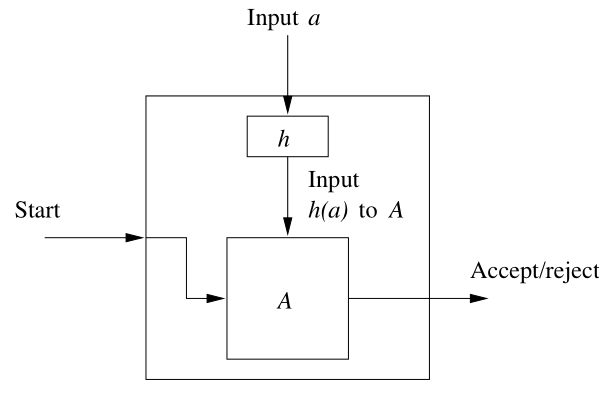
\includegraphics[scale=0.5]{files/inverseHomDFA.PNG}
    \end{center}
    \vspace{-24pt}\hfill\qedsymbol
    \begin{example}[Inverse homomorphism]
        $L'=L((\bf{00}+\bf{1})^*)$, $h(a)=01$, and $h(b)=10$: $h^{-1}(L')=(\bf{ba})^*$.
        [$h(L((\bf{ba})^*))\in L'$ is obvious, other words generate an isolated 0.]        
    \end{example}

\end{frame}


\section*{Decision properties of regular languages}


\begin{frame}{Testing emptiness}

    Given a representation of a regular language $L$, is $L=\emptyset$?

    \alert{FA:} is any final state reachable from the initial state? $O(n^2)$

    \alert{RE:} convert to $\epsilon-$NFA (in $O(n)$ time) and check reachability
    
    or directly: 
    
    \textbf{basis:} $\emptyset$ is empty, $\epsilon$ and $\bf{a}$ are not
    
    \textbf{induction:}
    \begin{itemize}
        \item $\alpha=(\alpha_1+\alpha_2)$: empty iff both $L(\alpha_1)$ and $L(\alpha_2)$ are empty
        \item $\alpha=(\alpha_1\alpha_2)$ empty iff either $L(\alpha_1)$ or $L(\alpha_2)$ is empty
        \item $\alpha=(\alpha_1^*)$ never empty, includes $\epsilon$            
    \end{itemize}

\end{frame}


\begin{frame}{Testing membership}

    Given a regular language $L$ and a word $w$, is $w\in L$?
    \begin{itemize}
        \item \alert{DFA:} run the automaton; if $|w|=n$, with a suitable representation (constant time transitions) it is in $O(n)$
        \item \alert{NFA} with $s$ states: running time $O(ns^2)$, each letter processed by taking the previous set of states
        \item \alert{$\epsilon$-NFA}: first compute the $\epsilon$-closure, then for each letter, process it and compute the $\epsilon$-closure of the result
        \item \alert{RE} of size $s$: convert to an $\epsilon$-NFA with at most $2s$ states and then simulate, $O(ns^2)$
    \end{itemize}

\end{frame}


\begin{frame}{Summary of finite automata}
\begin{itemize}
	\item Finite Automata: DFA, reduced DFA, NFA, $\epsilon$-NFA
    \item Regular Expressions
	\item Regular languages: closed under set operations, string operations, substitution, homomorphism, inverse hom.
	\item all FA and RE describe the same class of languages
	
	\item Key theorems
	
	\begin{itemize}
		\item Mihyll--Nerode (implicit DFA via congruences on words)
		\item Kleene (regular languages iff matched by RE)
		\item Pumping lemma
	\end{itemize}
\item (optional) 2-way automata
\item (optional) Automata with output
\begin{itemize}
	\item Moore machine
    \item Mealy machine.
\end{itemize}
\end{itemize}

\end{frame}


\begin{frame}{Summary of Lecture 4}

    \begin{itemize}
        \item regular expressions
        \item Kleene's theorem (two variants)
        \item constructions: RE to $\epsilon$-NFA, DFA to RE
        \item state elimination algorithm
        \item string substitution, homomorphism, inverse homomorphism
        \item decision properties
    \end{itemize}    

\end{frame}


\section*{Appendix: Visit every state}


\begin{frame}{Visit every state}

    \begin{example}[{visit every state}]
        Given a DFA $A$, let $L$ consist of all $w\in\Sigma^*$ that are accepted and, moreover, during the computation every state is visited, i.e.:
        \begin{itemize}
            \item $\delta^*(q_0,w)\in F$
            \item for every $q\in Q$ there is a prefix $x_q$ of $w$ s.t. $\delta^*(q_0,x_q)=q$
        \end{itemize}
        We will show that this language is regular.
    \end{example}
    Construct $L$ from $M=L(A)$ using operations preserving regularity:

    \begin{itemize}
        \item define an alphabet of `transitions': $T=\{[paq]\mid \delta(p,a)=q\}$
        \item define a homomorphism $h([paq])=a$ for all $p,q,a$
        \item $L_1=h^{-1}(M)$ is regular (inverse homomorphism), consists of accepting sequences of transitions
    \end{itemize}

\end{frame}


\begin{frame}{Visit every state: proof continues}

    \begin{itemize}
        \item start at $q_0$: $L_2=L_1\cap L(E_1.T^*)$, $E_1=\{[q_0aq]\mid a\in \Sigma, q\in Q\}$
        \item adjacent states must be equal: define non-matching pairs
        $$
        E_2=\{[paq][rbs]\mid q\neq r, p,q,r,s\in Q, a,b \in \Sigma\}$$
        and set $L_3=L_2-L(T^*.E_2.T^*)$ (remove if at least one non-matching pair of adjacent states)            
        \item $L_3$ already ends in accepting state: we started from $M=L(A)$
        \item all states: for $q\in Q$ let $E_q$ be the RE that is the sum of all the symbols in $T$ not containing $q$, set 
        $L_4=L_3-\bigcup_{q \in Q}\{L(E_q^*)\}$
        \item from a sequence of transitions back to the word: $L=h(L_4)$
    \end{itemize}\hfill\qedsymbol

\end{frame}


\end{document}

